First, we present the problem informally in the context of a case study to motivate the decentralized surveillance strategy synthesis procedure presented in this paper. We look at wildlife conservation in Africa. Specifically, we look at the Selous Game Reserve (SGR) located in Tanzania. A World Heritage Centre report released in 2013 \cite{UN13} outlines the seriousness of the threat to the African Black Rhinoceros population native to the SGR. Recommendations of the report include, inter alia, an anti-poaching initiative focused in the SGR. If a surveillance strategy can be synthesized for all the mobile sensors then the location of any potential poachers can be tracked to a user specified requirement. This will allow the authorities to narrow down the position of the target until the situation can be dealt with. 

Figure \ref{fig:casestudy} shows a section of the SGR that we represent as a gridworld which will form the states of the game. 

\begin{figure}
\subfloat[SGR interior landscape \cite{UN13} \label{fig:SGR-map}]{
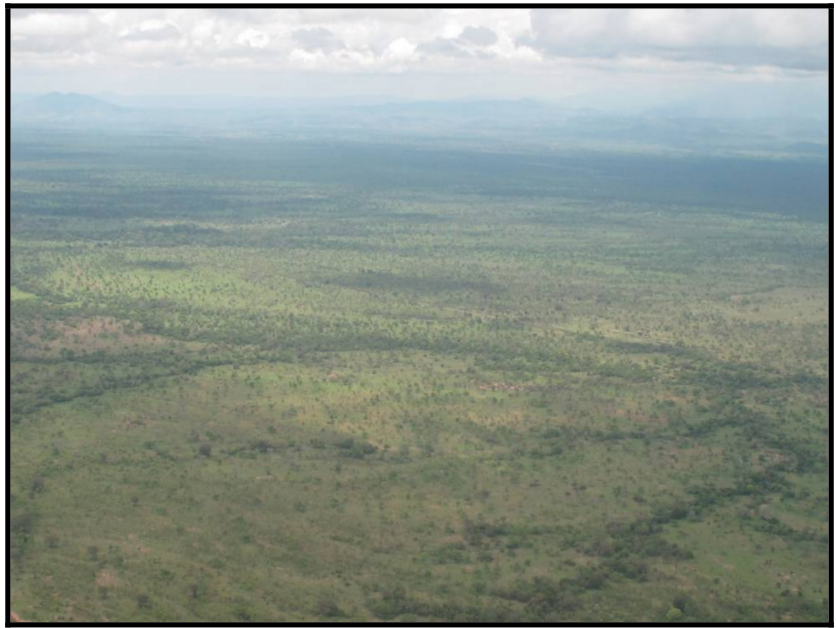
\includegraphics[scale=0.2]{figs/SGR.png}
\hspace{.3cm}}
%\hfill
\subfloat[Gridworld representation of landscape in \ref{fig:SGR-map} \label{fig:SGR-grid}]{
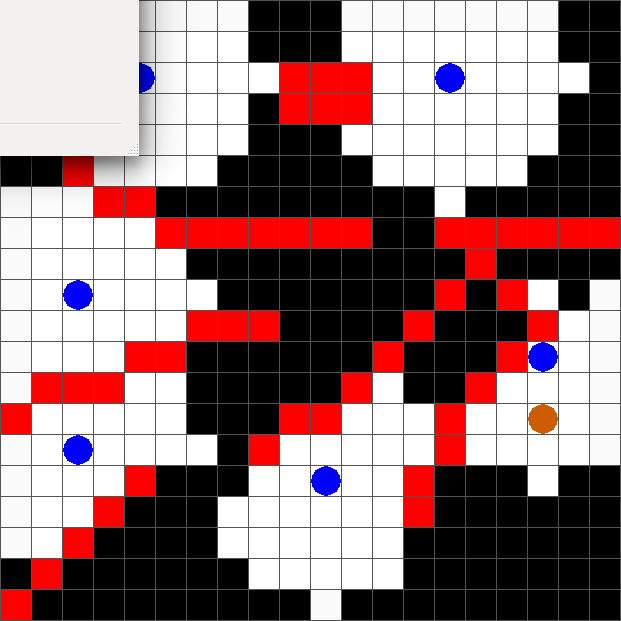
\includegraphics[scale=0.2]{figs/SGR-grid-vis.png}
}


\caption{The landscape in \ref{fig:SGR-map} is coarsely represented as a gridworld in \ref{fig:SGR-grid}. The mobile sensors or UAVs are blue circles and the target is represented in orange. The red cells represent impassable terrain (such as dense foliage) that also cannot be seen through by the sensors. Black cells are locations not visible to any sensor.}
\label{fig:casestudy}
\end{figure}

We model the mobile sensors as having an omnidirectional vision with limited range. Each static sensors have a set of states they can monitor. However, they are only able to detect the presence of a target in their set of states and cannot pinpoint the target's exact location. All the black states in the gridworld are states that are currently not in the range of any of the mobile sensors. 

 We want to compute a surveillance strategy that \emph{always eventually} brings the belief of the target location to within 5 cells. In other words, even if the target escapes vision of all the sensors, we want to guarantee that one of the sensors can bring the belief of the location of the target to less than 5 cells of the grid. 

In the next sections we present the definitions that will allow us to state this problem more formally.